In this lecture, we see two more problems that a quantum algorithm solves with far fewer queries than
any classical algorithm: the \emph{Bernstein--Vazirani} problem and \emph{Simon's problem}, the first
exponential quantum speed-up.

\paragraph{Recap: quantum queries and the Walsh--Hadamard transform.}

Both algorithms use the query
$U_f \colon \ket{x}\ket{b} \mapsto \ket{x}\ket{b \oplus f(x)}$ (\cref{fig:uf-0924}; one application is
one query) and the \emph{Walsh--Hadamard transform} (\cref{lem:wh-0924})
$H^{\otimes n} \ket{x} = \frac{1}{\sqrt{2^n}} \sum_{y \in \set{0,1}^n} (-1)^{x \cdot y} \ket{y}$, where
$x \cdot y = x_1 y_1 \oplus \dots \oplus x_n y_n$.

\begin{lemma}[Sum of Signs]\label{lem:signsum-0929}
    For every $z \in \set{0,1}^n$,
    \[\sum_{x \in \set{0,1}^n} (-1)^{z \cdot x} =
        \begin{cases}
            2^n & \text{if } z = 0^n, \\
            0   & \text{if } z \neq 0^n.
        \end{cases}\]
\end{lemma}

\begin{proof}
    If $z = 0^n$, all $2^n$ terms are $1$. If $z \neq 0^n$, pick $i$ with $z_i = 1$ and let $e_i$ be
    the string with a single $1$ in position $i$. The map $x \mapsto x \oplus e_i$ is its own inverse
    and has no fixed point, so it splits $\set{0,1}^n$ into $2^{n-1}$ disjoint pairs
    $\set{x, x \oplus e_i}$. The inner product is linear modulo $2$, so
    $z \cdot (x \oplus e_i) = z \cdot x \oplus z_i = z \cdot x \oplus 1$, and every pair contributes
    $(-1)^{z \cdot x} + (-1)^{z \cdot x \oplus 1} = 0$.
\end{proof}

In the Deutsch--Jozsa circuit (\cref{fig:dj-0924}, \cref{thm:dj-0924}) the query acts as the phase
flip $\ket{k} \mapsto (-1)^{f(k)} \ket{k}$, and the control register after the second layer of Hadamard
gates is in the state
\begin{equation}\label{eq:dj-state-0929}
    \sum_{y \in \set{0,1}^n} \alpha_y \ket{y},
    \qquad
    \alpha_y = \frac{1}{2^n} \sum_{k \in \set{0,1}^n} (-1)^{f(k) + k \cdot y}.
\end{equation}

\section{Bernstein--Vazirani Algorithm}

\begin{problem}[Bernstein--Vazirani Problem]
    Given $f \colon \set{0,1}^n \to \set{0,1}$ as a black box, with the \emph{promise} that
    \[f(x) = s \cdot x = s_1 x_1 \oplus s_2 x_2 \oplus \dots \oplus s_n x_n\]
    for some unknown $n$-bit string $s$, find $s$.
\end{problem}

\subsection{The Algorithm}

\begin{theorem}[Bernstein--Vazirani Algorithm]\label{thm:bv-0929}
    Run the Deutsch--Jozsa circuit (\cref{fig:dj-0924}) on $f(x) = s \cdot x$. Then measuring the $n$
    control qubits gives $y = s$ with probability $1$. So a single query finds $s$.
\end{theorem}

\begin{proof}
    By \cref{eq:dj-state-0929} (with the summation index $k$ renamed $x$), the control register is in
    the state $\sum_{y} \alpha_y \ket{y}$ with
    \[\alpha_y = \frac{1}{2^n} \sum_{x \in \set{0,1}^n} (-1)^{s \cdot x \oplus y \cdot x}
        = \frac{1}{2^n} \sum_{x \in \set{0,1}^n} (-1)^{(s \oplus y) \cdot x},\]
    because only the parity of the exponent matters and the inner product is bilinear modulo $2$. By
    \cref{lem:signsum-0929} with $z = s \oplus y$, $\alpha_y = 1$ if $y = s$ and $\alpha_y = 0$ if
    $y \neq s$. So the state is $\ket{s}$, and the measurement gives $s$ with probability $1$.
\end{proof}

\paragraph{Query complexity versus running time.} The query model only counts the calls to $U_f$. The
running time in the \emph{quantum Turing machine} (or quantum circuit) model counts all the gates.
The two are not always the same.

\section{Simon's Algorithm}

\begin{problem}[Simon's Problem]
    Given $f \colon \set{0,1}^n \to \set{0,1}^n$ as a black box, with the \emph{promise} that there is a
    string $s \in \set{0,1}^n$ such that for all $x, y$,
    \[f(x) = f(y) \iff x = y \text{ or } x = y \oplus s
        \qquad (\text{equivalently } s = x \oplus y),\]
    find $s$.
\end{problem}

If $s \neq 0^n$, then $f$ is \emph{$2$-to-$1$} with period $s$: the two inputs of a pair
$\set{x, x \oplus s}$ map to the same output, and different pairs map to different outputs. If
$s = 0^n$, then $f$ is \emph{$1$-to-$1$}. So the problem asks whether $f$ is $1$-to-$1$ or $2$-to-$1$
and, in the second case, for the period $s$. We write $N = 2^n$.

\paragraph{Query complexity.} Classically, Simon's problem needs $\bigOm{\sqrt{N}} = \bigOm{\sqrt{2^n}}$
queries, even for randomized algorithms (next lecture). Simon's quantum algorithm uses $\bigO{n}$
queries and a Gaussian elimination on an $n \times n$ system of linear equations over $\set{0,1}$,
which takes $\bigO{n^3}$ time. This is an exponential speed-up.

\subsection{The Circuit}

The circuit (\cref{fig:simon-0929}) has two registers of $n$ qubits each, all starting in $\ket{0}$.
Hadamard gates act on the control register before and after the single query $U_f$. Then the control
register is measured, giving a string $y \in \set{0,1}^n$. Because $f$ has $n$ output bits, we use
$U_f$ in its original form $\ket{x}\ket{b} \mapsto \ket{x}\ket{b \oplus f(x)}$ and not the phase flip
form.

\begin{figure}[ht]
    \centering
    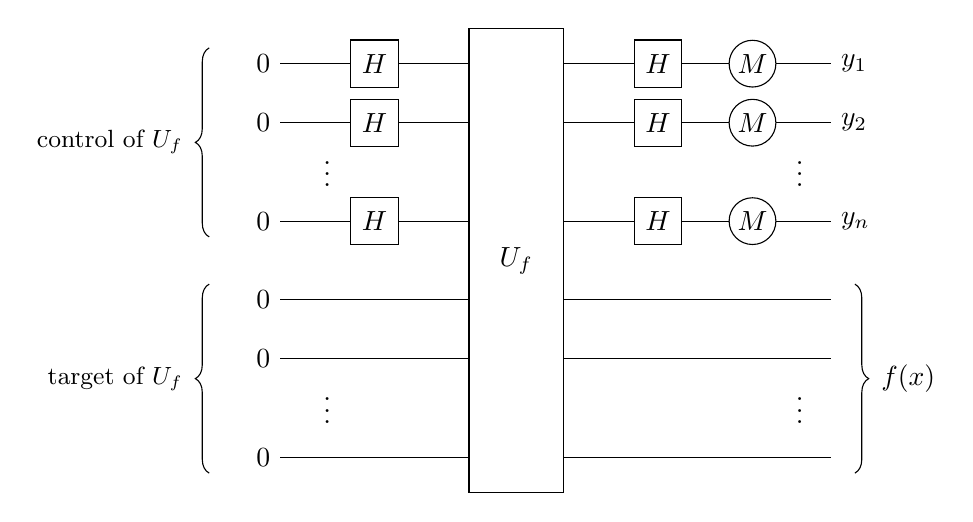
\begin{tikzpicture}[
            gate/.style={draw, fill=white, minimum size=6mm, inner sep=1pt},
            meter/.style={draw, circle, fill=white, inner sep=1.5pt},
        ]
        % control register
        \foreach \y in {4,3.25,2} {\draw (0,\y) -- (7,\y); \node[left] at (0,\y) {$\ket{0}$};}
        \node at (0.6,2.7) {$\vdots$};
        \node at (6.6,2.7) {$\vdots$};
        % target register
        \foreach \y in {1,0.25,-1} {\draw (0,\y) -- (7,\y); \node[left] at (0,\y) {$\ket{0}$};}
        \node at (0.6,-0.3) {$\vdots$};
        \node at (6.6,-0.3) {$\vdots$};
        % query
        \draw[fill=white] (2.4,-1.45) rectangle (3.6,4.45);
        \node at (3,1.5) {$U_f$};
        % Hadamard gates and measurements on the control register
        \foreach \y in {4,3.25,2} {
                \node[gate] at (1.2,\y) {$H$};
                \node[gate] at (4.8,\y) {$H$};
                \node[meter] at (6,\y) {$M$};
            }
        \node[right] at (7,4) {$y_1$};
        \node[right] at (7,3.25) {$y_2$};
        \node[right] at (7,2) {$y_n$};
        \draw[decorate, decoration={brace, amplitude=5pt, mirror}] (7.3,-1.2) -- (7.3,1.2)
        node[midway, right=6pt] {$\ket{f(x)}$};
        \draw[decorate, decoration={brace, amplitude=5pt}] (-0.9,1.8) -- (-0.9,4.2)
        node[midway, left=6pt] {\small control of $U_f$};
        \draw[decorate, decoration={brace, amplitude=5pt}] (-0.9,-1.2) -- (-0.9,1.2)
        node[midway, left=6pt] {\small target of $U_f$};
    \end{tikzpicture}
    \caption{Simon's circuit. The target register is not measured.}
    \label{fig:simon-0929}
\end{figure}

\subsection{Analysis of One Run}

\begin{theorem}[One Run of Simon's Circuit]\label{thm:simon-run-0929}
    Let $y$ be the string measured by the circuit of \cref{fig:simon-0929}.
    \begin{enumerate}
        \item If $f$ is $2$-to-$1$ with period $s \neq 0^n$, then $y$ is uniformly distributed over the
              $2^{n-1}$ strings $y$ with $s \cdot y = 0$: each of them has probability $\sfrac{1}{2^{n-1}}$,
              and every $y$ with $s \cdot y = 1$ has probability $0$.
        \item If $f$ is $1$-to-$1$, then $y$ is uniformly distributed over all of $\set{0,1}^n$: each
              string has probability $\sfrac{1}{2^n}$.
    \end{enumerate}
\end{theorem}

\begin{proof}
    By \cref{lem:wh-0924}, the first layer of Hadamard gates gives
    $\frac{1}{\sqrt{2^n}} \sum_{x} \ket{x}\ket{0^n}$. The query $U_f$ turns this into
    $\frac{1}{\sqrt{2^n}} \sum_{x} \ket{x}\ket{f(x)}$. The second layer of Hadamard gates on the
    control register (\cref{lem:wh-0924} applied to every $\ket{x}$) gives
    \begin{equation}\label{eq:simon-final-0929}
        \frac{1}{2^n} \sum_{y \in \set{0,1}^n} \sum_{x \in \set{0,1}^n} (-1)^{x \cdot y} \ket{y}\ket{f(x)}.
    \end{equation}
    The amplitude $\alpha_{y,z}$ of a basis state $\ket{y}\ket{z}$ collects the $x$ with $f(x) = z$.
    Measuring only the first register gives $y$ with probability $\sum_{z} \abs{\alpha_{y,z}}^2$
    (the probabilities of all basis states $\ket{y}\ket{z}$ with this $y$ add up).

    \emph{Case 2: $f$ is $1$-to-$1$.} The $2^n$ strings $f(x)$ are all different, so every basis state
    $\ket{y}\ket{f(x)}$ appears exactly once in \cref{eq:simon-final-0929}, with amplitude
    $\frac{1}{2^n} (-1)^{x \cdot y}$. So $y$ has probability
    $\sum_{x} \abs{\frac{1}{2^n} (-1)^{x \cdot y}}^2 = 2^n \cdot \frac{1}{2^{2n}} = \frac{1}{2^n}$.

    \emph{Case 1: $f$ is $2$-to-$1$ with period $s \neq 0^n$.} The range $R$ of $f$ has
    $\abs{R} = 2^{n-1}$ elements. For every $z \in R$ let $x_z$ be one of its two preimages; the other
    is $x_z \oplus s$. Because $(x_z \oplus s) \cdot y = x_z \cdot y \oplus s \cdot y$, the amplitude of
    $\ket{y}\ket{z}$ in \cref{eq:simon-final-0929} is
    \[\frac{1}{2^n} \left((-1)^{x_z \cdot y} + (-1)^{(x_z \oplus s) \cdot y}\right)
        = \frac{1}{2^n} (-1)^{x_z \cdot y} \left(1 + (-1)^{s \cdot y}\right)\]
    for $z \in R$ (and $0$ for $z \notin R$). So $y$ has probability
    \[\sum_{z \in R} \abs{\frac{1}{2^n} \left(1 + (-1)^{s \cdot y}\right)}^2
        = 2^{n-1} \cdot \frac{\left(1 + (-1)^{s \cdot y}\right)^2}{2^{2n}}
        = \begin{cases}
            \sfrac{1}{2^{n-1}} & \text{if } s \cdot y = 0, \\
            0                  & \text{if } s \cdot y = 1.
        \end{cases}\]
    There are $2^{n-1}$ strings $y$ with $s \cdot y = 0$, because the pairing $y \mapsto y \oplus e_i$
    of the proof of \cref{lem:signsum-0929}, with $s_i = 1$, matches every $y$ with $s \cdot y = 0$ to
    a $y'$ with $s \cdot y' = 1$.
\end{proof}

\subsection{From the Measurements to \texorpdfstring{$s$}{s}}

Each run of the circuit gives a random $y$ with $s \cdot y = 0$, which is one linear equation
$s_1 y_1 \oplus s_2 y_2 \oplus \dots \oplus s_n y_n = 0$ for the unknown bits $s_1, \dots, s_n$. Running
the circuit $n - 1$ times gives a homogeneous system
\[y_1 \cdot s = 0, \quad y_2 \cdot s = 0, \quad \dots, \quad y_{n-1} \cdot s = 0\]
of linear equations over the field $\set{0,1}$ (addition is $\oplus$). If $y_1, \dots, y_{n-1}$ are
\emph{linearly independent} over $\set{0,1}$, the system has rank $n - 1$. Then its solution space has
dimension $n - (n-1) = 1$ and consists of $0^n$ and one nonzero string $s'$. Gaussian elimination over
$\set{0,1}$ tests the independence and computes $s'$ in $\bigO{n^3}$ time. The true $s$ satisfies every
equation. So if $s \neq 0^n$, at most $n - 1$ of them can be independent, and $n - 1$ independent ones
are enough: if the $y_i$ are independent and $f$ is $2$-to-$1$, then $s' = s$.

\begin{algorithm}[ht]
    \caption{Simon's algorithm}
    \label{alg:simon-0929}
    \begin{algorithmic}[1]
        \State run the circuit of \cref{fig:simon-0929} $n - 1$ times; let $y_1, \dots, y_{n-1}$ be the measured strings
        \If{$y_1, \dots, y_{n-1}$ are linearly dependent over $\set{0,1}$} \Comment{Gaussian elimination}
        \State \Return \textsc{fail}
        \EndIf
        \State let $s'$ be the unique nonzero solution of $y_1 \cdot s' = \dots = y_{n-1} \cdot s' = 0$
        \If{$f(s') = f(0^n)$} \Comment{two classical queries}
        \State \Return $s'$ \Comment{$f$ is $2$-to-$1$ with period $s'$}
        \Else
        \State \Return $0^n$ \Comment{$f$ is $1$-to-$1$}
        \EndIf
    \end{algorithmic}
\end{algorithm}

\begin{theorem}[Simon's Algorithm]\label{thm:simon-0929}
    \cref{alg:simon-0929} makes $n + 1$ queries ($n - 1$ quantum, $2$ classical) and $\bigO{n^3}$ other
    operations. It never outputs a wrong answer, and it outputs the correct $s$ with probability at least
    $\sfrac{1}{4}$.
\end{theorem}

\begin{proof}
    \emph{Never wrong.} If the algorithm does not fail, $y_1, \dots, y_{n-1}$ are independent and $s'$
    is the unique nonzero solution of the system. If $f$ is $2$-to-$1$ with period $s$, then $s$ is a
    nonzero solution, so $s' = s$. The test $f(s') = f(0^n) = f(0^n \oplus s)$ succeeds, and the output
    $s' = s$ is correct. If $f$ is $1$-to-$1$, then $f(s') \neq f(0^n)$ because $s' \neq 0^n$, and the
    output $0^n = s$ is correct.

    \emph{Success probability.} The algorithm fails only if the $y_i$ are dependent. The $n - 1$ runs are
    independent (the registers are re-initialized to $\ket{0^n}\ket{0^n}$ for every run). By
    \cref{thm:simon-run-0929}, the $y_i$ are independent uniform samples from the $2^{n-1}$ strings with
    $s \cdot y = 0$ if $f$ is $2$-to-$1$, and from all of $\set{0,1}^n$ if $f$ is $1$-to-$1$. By
    \cref{thm:indep-1001} (next lecture) they are linearly independent with probability
    \[\left(1 - \frac{1}{2}\right)\left(1 - \frac{1}{2^2}\right)\left(1 - \frac{1}{2^3}\right) \cdots \left(1 - \frac{1}{2^{n-1}}\right) \geq \frac{1}{4}\]
    in the first case and at least $\sfrac{1}{2}$ in the second.
\end{proof}

\subsection{A Deterministic Classical Algorithm}

\begin{exercisebox}
\begin{exercise}\label{ex:simon-det-0929}
    Find a deterministic classical algorithm for Simon's problem that makes $\bigO{\sqrt{2^n}}$ queries.
\end{exercise}
\tcblower
\begin{wsolution}
    We query a set $S$ such that every nonzero string is the XOR of two elements of $S$. A collision
    in $S$ then gives $s$. Let $m = \ceil{n/2}$ and write every $n$-bit string as $x = (u, v)$ with
    $u \in \set{0,1}^m$ its first $m$ bits and $v \in \set{0,1}^{n-m}$ its last $n - m$ bits. Let
    \[S_1 = \set{(u, 0^{n-m}) \suchthat u \in \set{0,1}^m}, \qquad
        S_2 = \set{(0^m, v) \suchthat v \in \set{0,1}^{n-m}}, \qquad
        S = S_1 \cup S_2.\]

    \emph{The algorithm.} Query $f$ on every $x \in S$. If there are $x \neq x'$ in $S$ with
    $f(x) = f(x')$, output $s = x \oplus x'$. Otherwise output $s = 0^n$.

    \emph{Queries.} Because $n - m \leq m \leq \sfrac{(n+1)}{2}$, the algorithm makes
    $\abs{S} \leq 2^m + 2^{n-m} \leq 2 \cdot 2^{m} \leq 2 \cdot 2^{(n+1)/2} = 2\sqrt{2} \cdot \sqrt{2^n}
        = \bigO{\sqrt{2^n}}$ queries, and it is deterministic.

    \emph{Claim: every $s \neq 0^n$ is the XOR of two different elements of $S$.} Write $s = (u, v)$. Then
    $(u, 0^{n-m}) \in S_1$, $(0^m, v) \in S_2$ and $(u, 0^{n-m}) \oplus (0^m, v) = s$. The two elements
    are different, because otherwise $u = 0^m$ and $v = 0^{n-m}$, so $s = 0^n$.

    \emph{Correctness.} If $f$ is $2$-to-$1$ with period $s \neq 0^n$, by the claim there are $x \neq x'$
    in $S$ with $x' = x \oplus s$, so $f(x) = f(x')$ and we find a collision. Any collision
    $f(x) = f(x')$ with $x \neq x'$ satisfies $x' = x \oplus s$ by the promise, so the output
    $x \oplus x' = s$ is correct. If $f$ is $1$-to-$1$ there is no
    collision, and the output $0^n = s$ is correct.
\end{wsolution}
\end{exercisebox}
